\begin{itemize}
    \item A trigger is basically is a block of SQL code that will define what needs to happen when a certain operation gets performed on a database.
    
    \item Lets create a table called \verb|trigger_test| to store the trigger calls.
        \begin{minted}[autogobble]{sql}
            CREATE TABLE trigger_test (
                message VARCHAR(100)
            );
        \end{minted}

    \item Making a trigger needs to be done from the command line.
        \begin{minted}[autogobble]{sql}
            DELIMITER $$ 
            CREATE 
                TRIGGER my_trigger BEFORE INSERT 
                ON employee
                FOR EACH ROW BEGIN 
                    INSERT INTO trigger_test VALUES('added new people');
                END$$
            DELIMITER ;
        \end{minted}
        \begin{verbatim}
            Enter password: ********
            Welcome to the MySQL monitor.  Commands end with ; or \g.
            Your MySQL connection id is 10
            Server version: 8.0.22 MySQL Community Server - GPL

            Copyright (c) 2000, 2020, Oracle and/or its affiliates. All rights reserved.

            Oracle is a registered trademark of Oracle Corporation and/or its
            affiliates. Other names may be trademarks of their respective
            owners.

            Type 'help;' or '\h' for help. Type '\c' to clear the current input statement.

            mysql> DELIMITER $$
            mysql> CREATE
                -> TRIGGER my_trigger BEFORE INSERT
                -> ON employee
                -> FOR EACH ROW BEGIN
                ->   INSERT INTO trigger_test VALUES('added new people');
                -> END$$
            Query OK, 0 rows affected (0.03 sec)
            mysql> DELIMITER ;
        \end{verbatim}
        \begin{itemize}
            \item Now we can see a message whenever we make the specified action, in this case inserting Oscar Martinez and then using select statements see the registered actions in the table ``trigger\_test''.
        \end{itemize}
        \begin{minted}[autogobble]{sql}
            INSERT INTO employee VALUES(109, 'Oscar', 'Martinez', '1968-02-19', 'M', 69000, 106, 3);
            SELECT * FROM trigger_test;
        \end{minted}
        \begin{figure}[H]
            \centering
            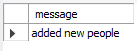
\includegraphics[width=0.4\textwidth]{./Figs/2020-12-24-22-16-41.png}
        % 	\caption{}
        \end{figure}
    
    \item We now want to store the first name in the trigger test table.
        \begin{minted}[autogobble]{sql}
            DELIMITER $$
            CREATE
                TRIGGER my_trigger1 BEFORE INSERT
                ON employee
                FOR EACH ROW BEGIN
                    INSERT INTO trigger_test VALUES(NEW.first_name);
                END$$
            DELIMITER ;
        \end{minted}
        \begin{verbatim}
            Enter password: ********
            Welcome to the MySQL monitor.  Commands end with ; or \g.
            Your MySQL connection id is 10
            Server version: 8.0.22 MySQL Community Server - GPL

            Copyright (c) 2000, 2020, Oracle and/or its affiliates. All rights reserved.

            Oracle is a registered trademark of Oracle Corporation and/or its
            affiliates. Other names may be trademarks of their respective
            owners.

            Type 'help;' or '\h' for help. Type '\c' to clear the current input statement.

            mysql> DELIMITER $$
            mysql> CREATE
                -> TRIGGER my_trigger1 BEFORE INSERT
                -> ON employee
                -> FOR EACH ROW BEGIN
                ->    INSERT INTO trigger_test VALUES(NEW.first_name);
                -> END$$
            Query OK, 0 rows affected (0.03 sec)
            mysql> DELIMITER ;
        \end{verbatim}
        \begin{itemize}
            \item Using select statements we can see the registry the trigger has left when inserting Kevin Malone.
        \end{itemize}
        \begin{minted}[autogobble]{sql}
            INSERT INTO employee VALUES(110, 'Kevin', 'Malone', '1978-02-19', 'M', 69000, 106, 3);
            SELECT * FROM trigger_test;
        \end{minted}
        \begin{figure}[H]
            \centering
            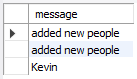
\includegraphics[width=0.4\textwidth]{./Figs/2020-12-24-22-23-15.png}
        % 	\caption{}
        \end{figure}

    
    \item Example:
        \begin{minted}[autogobble]{sql}
            DELIMITER $$ 
                CREATE TRIGGER my_trigger2 BEFORE INSERT 
                ON employee 
                FOR EACH ROW BEGIN 
                    IF NEW.sex = 'M' THEN 
                        INSERT INTO trigger_test VALUES('added male employee');
                    ELSEIF NEW.sex = 'F' THEN 
                        INSERT INTO trigger_test VALUES('added female');
                    ELSE 
                        INSERT INTO trigger_test VALUES('added other employee');
                    END IF;
                END$$
            DELIMITER ;
        \end{minted}
        \begin{verbatim}
            Enter password: ********
            Welcome to the MySQL monitor.  Commands end with ; or \g.
            Your MySQL connection id is 10
            Server version: 8.0.22 MySQL Community Server - GPL

            Copyright (c) 2000, 2020, Oracle and/or its affiliates. All rights reserved.

            Oracle is a registered trademark of Oracle Corporation and/or its
            affiliates. Other names may be trademarks of their respective
            owners.

            Type 'help;' or '\h' for help. Type '\c' to clear the current input statement.

            mysql> DELIMITER $$
            mysql> CREATE TRIGGER my_trigger2 BEFORE INSERT 
                -> ON employee 
                -> FOR EACH ROW BEGIN 
                ->     IF NEW.sex = 'M' THEN 
                ->         INSERT INTO trigger_test VALUES('added male employee');
                ->     ELSEIF NEW.sex = 'F' THEN 
                ->         INSERT INTO trigger_test VALUES('added female');
                ->     ELSE 
                ->         INSERT INTO trigger_test VALUES('added other employee');
                ->     END IF;
                -> END$$
            Query OK, 0 rows affected (0.03 sec)
            mysql> DELIMITER ;
        \end{verbatim}
        \begin{itemize}
            \item Using select statements we can see the registry the trigger has left when inserting Pam Beesly.
        \end{itemize}
        \begin{minted}[autogobble]{sql}
            INSERT INTO employee VALUES(111, 'Pam', 'Beesly', '1988-02-19', 'F', 69000, 106, 3);
            SELECT * FROM trigger_test;
        \end{minted}
        \begin{figure}[H]
            \centering
            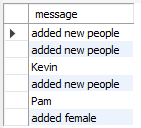
\includegraphics[width=0.4\textwidth]{./Figs/2020-12-24-22-24-04.png}
        % 	\caption{}
        \end{figure}
    
    \item Use \mintinline{sql}{DROP TRIGGER} command to eliminate the trigger.
\end{itemize}
